\chapter{Context théoritique}

\label{ch:contexte}

\section{Introduction}

In this part we will unwrap some mathematical notions of the theory behind Phase Vocoders. To embrace the theory of spectral dissolution, one has to accept that a complex signal, meaning something more than a single sine wave, can be representated through a series of overlaps of simple sinusoids with different amplitudes and frequencies.

To visualize this method the paradigm of additive synthesis should be used as an inverse construction. A classic method of synthesizing a complex time-varying sound consists of combining a number of elementary waveforms. The waveforms that are superimposed in additive synthesis are often sinusoidal. Under certain conditions, the individual sinusoids fuse together and the result is perceived as a single rich sound.

The idea behind this method is not new. Indeed, additive synthesis has been used for centuries in traditional instruments such as organ.

When an almost-periodic sound is analyzed, its spectral energy is concentrated around a few discrete frequencies (Harmoniques). These frequency lines correspond to different sunisoidal signals called partiels. The amplitude of each partial is not constant and and its time-variation is critical for timbral characterisation. Indeed, in the initial transistory phase(attack) of a note. The frequency of each component, however, can be thought of as slowly varying. Additive synthesis consists of the sum of sinusoidal oscillators whose amplitude and frequency are time varying. The control parameters are determined through spectral analysis.



\section{Mathematical Decoding}


%------------------------------Fourier TRANSFORM-------------------------------



\subsection{The Fourier Transform}

Spectral analysis is essentially the process of passing from the temporal domain to the frequency domain for a fixed time period. From this point of view, spectral analysis, is a fourrier transformation together with some mathematical processing that allow the visualization of the frequencies that compose a complex sound wave for a fixed time period.

There are many way to compute the Discrete Fourier Transform (DFT)one of which is the FFT. Allthough all the DFT methods convert to same result, the FFT is one of the most efficient computationally. FFT is one of the most used algorithms in signal processing due to the minimal amount of code necessary to program it. Nevertheless, it's among the most difficult algorithms in the DSP domain.

FFT is a complex algorithm, in the sence that it uses complex numbers to compute. Due to its complexity the technical details are frequently omited and left to a more mathematical crowd.

The process of DFT is graphically explained in figure \ref{ComplexDFT}. In the left column, one can see the temporal representation of the signal. Accordingly, in the right column the FFT transformation can be visualized in the frequency domain. $N$ is the window size in DSP terms or the total duration of the analysis in general. As it is shown in the figure \ref{ComplexDFT}, the signal is decomposed in 2-axe variables, a real and an imaginary.


\begin{figure}
    \centering
    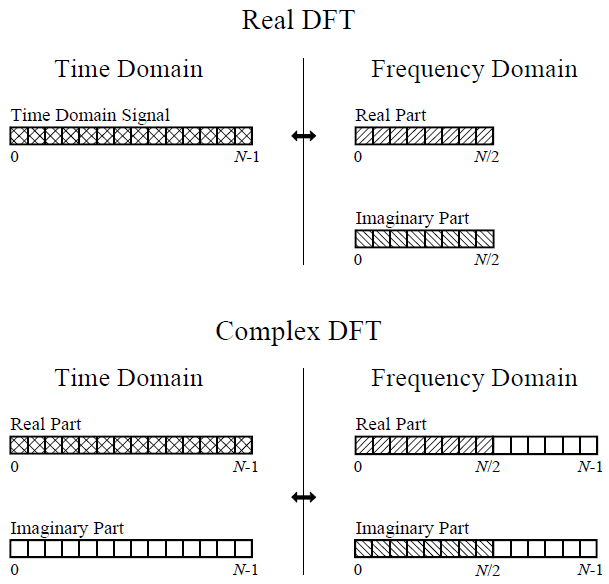
\includegraphics[width = 0.5 \textwidth ]{Graphs/ComplexDFT.png}
    \caption{Complex DFT}
    \label{ComplexDFT}
\end{figure}




%-------------------------------État de travail-----------------
In 1822 Jean Joseph Fourier showed that some semi-periodic functions can be formulated as a sum of harmonics likewise : 

%La fonction périodique de Fourier peut être formée comme ci-dessous :
 
\begin{equation}\footnote{Curtis Roads. The Computer Music Tutorial. MIT Press, Cambridge, MA, USA, 1996. ISBN 0262680823.[p. 1085]}
    x(t) = c_0 + \sum_{n=1} ^ \infty c_n cos( \omega t + \theta_n) 
\end{equation}

Where $t$ is the time period, $x$ is the signal, $c_0$ is the fundamental harmonic, $f$ the frequency, $\omega = 2 \pi f$ and $\theta$ is the phase of every harmonic. In this formulation of the Fourier transform is clear that a sound $x$ bounded of the time factor $t$ can be described as a sum of sinusoids.

% Ou $t$ est le temps, $x$ le signal sonore, $c_0$ l'harmonique fondamentale, $f$ la fréquence, $\omega = 2 \pi f$ et $\theta_n$ la phase de chaque harmonique. Dans cette formulation de la transformation Fourier il est clair que un son $x$ dépendant de temps $t$ peut être interprété comme une somme des sinusoïdes.

Thus, the Fourier transform for any intergatable function $f: \mathbb{R} \to \mathbb{C}$ is the written as follows :

% En revanche, la formule générale de la transformation Fourrier est la suivante :
 
\begin{equation}\footnote{Hermann L F. Helmholtz. The Sensations of Tone. New York, 1895.[p. 215]}
     F[x(t)](\omega) = \int_{-\infty}^{+\infty} e ^ {-j \omega t} x(t) \hspace{1mm} dt \hspace{5mm} 
\end{equation}
    
Where $F[x(t)](\omega)$ is the Fourier transformation of the signal $x$ bounded by a frequency $\omega$. In sound the this frequency is varied between 0 and the Sample Rate (SR). The SR is usually 44100 or 48000Hz. The Kernel of the intergatable function for digital sound signals varies into the integral $[-1, 1]$. As it is clear to see in this formula the time functor is infinite, but computationaly this is obviously imposible. Other variations of the Fourier transform in discrete time are actually used in computer science.

% Ou $F[x(t)](\omega)$ est la transformation Fourrier du signal $x$ dépendante à une fréquence variée $\omega$. Dans le domaine sonore cette fréquence se varie entre 0 et le SR\footnote{SR = Sampling Rate ou fréquence d'échantillonage en français. Suivant 44100 ou 48000Hz}. 

% Explication Graphique
         \begin{figure}
            \centering
            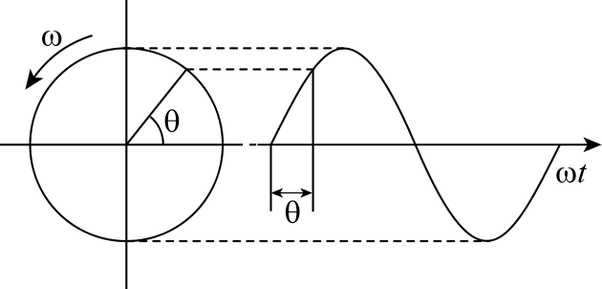
\includegraphics[width = 0.5 \textwidth ]{Graphs/Fourier_Circle_1.png}
            \caption{Circle de la transformation Fourier}
            \label{CircleFourier}
        \end{figure}

The Fourier transform is based primarily on Eulers formula where $e ^ {2 j \pi t} = cos(2 \pi t) + j sin(2 \pi t)$. One can imagine this operation as drawing of a circle in the complex plane $\mathbb{C}$. During the fourier transformation a signal $x(t)$ is rendered around a circle with ($e ^ {- j \omega t}$), with a frequency $f$. Remember that $\omega = 2 \pi f$. The rotation is given by the sign of $j$. A clockwise rotation is considered thus $-j$. This process gives us effectively two parts the real, $cos( 2 \pi t)$, and the imaginary, $j \; sin(2 \pi t)$,  part of the equation.


One would often transform the cartesian data induced by the complex exponential to a more signal familiar pollar form. After the Fourier transform, there are two factor to manipulate, phase and magnitude. Phase is induced by the angle of the two cartesian coordinates in the complex plane while magnituded is deducted by the produced vector of the two values. From the phase one can extract information about the frequency of the signal in the precise bin and, as the name implies, from magnitude information about the amplitude of the exact bin. When the time is fixed for the perform of Fourier analysis, then the sound signal is divised into frequency bins factorized by the frequency of the analysis ($\omega$). The phase and the magnitude are calculated for each fraction of time on which Fourier analysis is performed. The magnitude is equal to : $m(x) = \sqrt{i(x)^2 + r(x)^2}$ and the phase is $\theta(x) = tan^{-1}(\frac{i(x)}{r(x)})$. \ref{MagnitudePhase}


         \begin{figure}
            \centering
            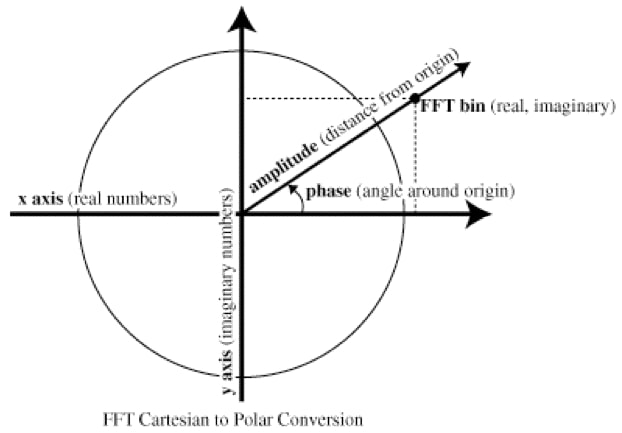
\includegraphics[width = 0.5 \textwidth ]{Graphs/Fourier_Circle_2.jpg}
            \caption{Magnitude et phase}
            \label{MagnitudePhase}
        \end{figure}

Evidently in the digital domain one cannot use an infinite time portion. Thus we introduce the notion of the window and analogically windowing. The window is a period of time expressed in frames. Frames is an equivalent notion to SR in the sense that the SR calculated an amount of images of the sound per minute and the frames are exactly these images.  A windowed analysis is usually expressed by a Short Time Fourier Transform (STFT) algorithm \footnote{STFT : Short Time Fourier Transform, Jown Strawn. Introduction to digital sound synthesis. Digital Audio Engineering, pages 141–
134, 1985.}.


\begin{equation}
\footnote{Tadej Droljc. STFT Analysis Driven Sonographic Sound Processing in Real-Time using Max/MSP and Jitter. 2011.}
    X(\omega, \tau) = \sum_t ^ \infty x(t) \omega(t-\tau)e ^ {-j \omega t} \hspace{5mm} 
\end{equation}

Where $x$ represents the signal, $X$ it's Fourier transform (an abreviation of $F[x(t)]$), $\omega = 2 \pi f$ , $t$ is the continuous time, $\tau$ is the instant time, $c_n$ the harmonics. $\omega(t)$ the windowing and $j$ a the complex constant value. 

Où $x$ est le signal, $X$ sa transformée Fourier (une abréviation de la forme $F[x(t)]$), $\omega = 2 \pi f$ , $t$ le temps continue, $\tau$ l’instant temporel, $c_n$ l’harmoniques, $\omega(t)$ le fenêtrage, et $j$ un nombre complexe.

Dans cette recherche, on va utiliser la forme continue TFD et puis FFT, vu que cette formule est premièrement utilisée dans MaxMSP et en plus requiert une puissance calculatrice plus efficiente que d’autres méthodes  :    

As mentioned above, MaxMSP uses a FFT algorithm. It is among the most efficient algorithms for Fourier analysis.

\begin{equation}
\footnote{Jean-François Charles. A tutorial on spectral sound processing using maxmsp and jitter. Computer Music Journal, pages 87–102, Printemps 2008.}
    X(\omega) = \frac{1}{N} \sum_{n = 0} ^ {N-1} x(n+1) e ^ {-j \frac{\omega n}{N}} \hspace{5mm}
\end{equation}

Where $N$ is the size of the window, which is the total amount of frames it contains.$x$ is the signal, $n$ enumerates every frame in $N$ and $\omega = 2 \pi f$ as usual but in this version f is varied between 0 and N. We will rather present it as $\omega = 2 \pi k$ where k will represent the $k-$harmonic.

%Ou $N$ est la totalité des instants sonores échantillonnés de notre signal $x$, $n$ signifie chauque instant sonore, et $\omega = 2 \pi f$ est toujour la frequence variée.

For every transition to the frequency domain, a inverse function to the temporal domain is necessary. The inverse function is caracterized as Inverse Fast Fourier Transform (IFFT) for discrete time values.

%Pour chaque transition au domaine frequentiel, il faut une tranformation retour au domaine temporel. Le resultat est caracterisé comme la tranformation Fourier inverse (IFFT).

\begin{equation}
\footnote{Alan V. Oppenheim et Ronald W. Schafer. Discrete-time signal processingd. Prentice Hall Press.}
    x(n) = \frac{1}{N} \sum_{ f = 0} ^ {N-1} X(f) e ^ {j \frac{2 \pi f n}{N}} \hspace{5mm} 
\end{equation}
 
 %------------------------------FENÊTRAGE-------------------------------

\subsubsection{Fast Fourier Transform}

It's always fine to have a theorical basepoint but what really matters is computational formulas. By computational we mean I formula that is easy to be executed by a computer and produce an output. A solution to this statement is Fast Fourier Transform. Thus, FFT is a computable algorithm for DFT that uses a smart way to reduce the time of the computation and the complexity of the calulations.

We remind the standard DFT intepreted in computable code.

    \begin{lstlisting}[language=Python, caption= DFT]
    function DFT(x)
        N = length(x)
        # We want two vectors here for real space (n) and frequency space (k)
        n = 0:N-1
        k = n'
        transform_matrix = exp.(-2im*pi*n*k/N)
        return transform_matrix*x
    end.
    \end{lstlisting}

It's clear to see that the Fourier transform is actually a computation matrix. However, but performing that much computation one can imagine that the process is quite slow. The requirements for DFT are real-time processing and windows of minimum size 512 samples for sound data. The improvement of the algorithm was given by James Cooley and John Tukey \footnote{James Cooley et John Tukey, \textit{An algorithm for the machine calculation of complex Fourier series}, 1965. \nocite{Fourier_complex}}
 
The Cooley-Tukey algorithm uses recursion to reduce the computational complexity. In particular, the matrix produced by the reduction to frequency domain is reduced into two parts before performing the DFT calculations. We seperate the odd indices of the bins from the even and then the procedure is repeated. This process reduces the complexity to $\mathcal{O}(n \; log \; n)$ from a polynomial size. Ofcourse to perform this action due to continuous division by two we require the analysis window to be a power of two. 

The core of the FFT calculation reduction are butterfly diagrams. In particular, Cooley and Tukey noticed that complex exponential is entirely repeated in the second half of the window with an opposite sign. Therefore, by constantly dividing the video the calculations of the complex exponential are vastly reducted. We can visualize the process in the figure \ref{Butterfly} \footnote{Image recuperé de l'article : \href{https://www.researchgate.net/figure/Radix-2-butterfly-diagram-for-8-point-FFT_fig1_312460770}{P. G. Reshma, P. Gopi Varun, Babu V. Suresh, Wahid Khabou, \textit{Analog CMOS implementation of FFt using cascode current mirror}, 2017.}}.

    \begin{figure}
        \centering
        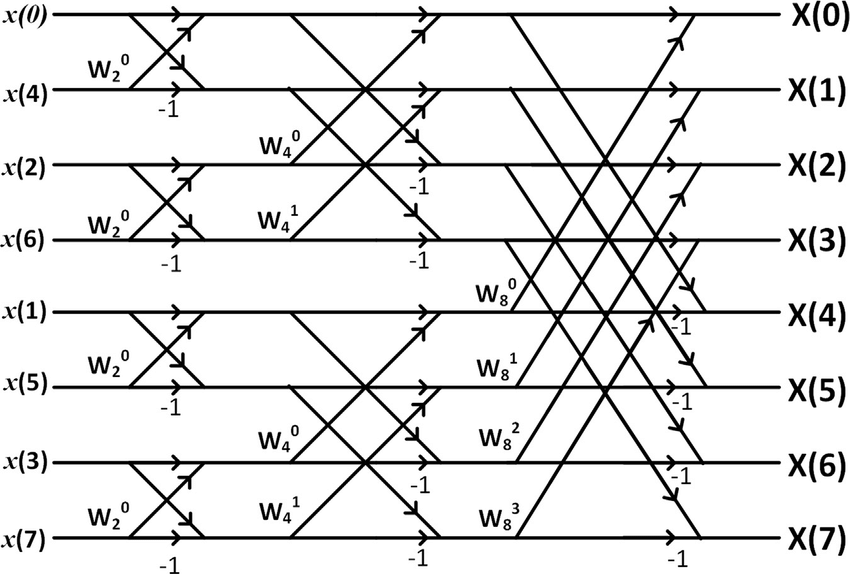
\includegraphics[width = 8cm]{Graphs/Butterfly_8-point-FFT.png}
        \caption{Butterfly Diagrams for an 8 point FFT}
        \label{Butterfly}
    \end{figure}

A code implementation of this method can be find in the Appendix \ref{Cooley-Tukey_Code}.

\subsection{Windowing}

 %Explaining overlapping and windowing
To calculate the STFT, one must define the size of the window to be processed. The fourier transform in a discrete time window may produce artificacts contradicting the continum of the signal. To prevent this it is customary to multiply the window of the original sound with a default window of the same size on which a default function factorizes the amplitude of the sound. The Fourier transform is reproduced countably many times in relation of the size of the sound analyzed. The window is usually significantly smaller than the original sound itself, thus it repeated multiple times throughout the duration of the sound. It is important that the window is moved temporally but it is also overllaped by a fuctor to itself. The process can be visually described in the figure \ref{overlapping}.

This technique, named overlapping, renders a round sound result. Due to overlapping and the envellop multiplication the listener cannot perceive any possible artifacts induced by the analysis but one hears a unified result \footnote{Daniel W. Griffin et Jae S. Lim. Signal estimation from modified short-time fourier transform. IEE Transaction on acoustics, speech, and signal processing, ISSE Vol. 32 :236–243, Avril 1984.}. 

 
Comme il a été déjà mentionné, pour calculer une STFT, une fenêtre d’une certaine durée est nécessaire pour être définie. Pour cette fenêtre, une certaine fonction peut être appliquée pour éviter les cliques comme (hanning, hamming, exponentielle, etc). Pendant STFT, il est habituel de
chevaucher les fenêtres l’un dans l’autre. Cette procédure est expliquée graphiquement dans la figure \ref{overlapping}.

Cette technique, nommée overlapping, nous permet de créer un résultat lisse au niveau sonore. Lors
de changement de fenêtres l’auteur ne peut pas percevoir que le son était décomposer en morceaux
mais il attend un résultat sonore unifié \footnote{Daniel W. Griffin et Jae S. Lim. Signal estimation from modified short-time fourier transform. IEE Transaction on acoustics, speech, and signal processing, ISSE Vol. 32 :236–243, Avril 1984.}. 

%Explain Windowing musically
 
 
         \begin{figure}
            \centering
            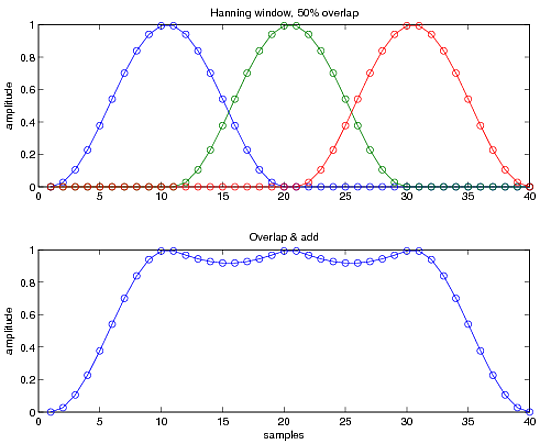
\includegraphics[width = 0.5 \textwidth ]{Graphs/Overlapping.png}
            \caption{Overlapping}
            \label{overlapping}
        \end{figure}

\subsubsection{Gabor Filters}

Here we will examine the possibility of using Gabor filters to envellop the signal. Gabor filters are defined as the continuous multiplication of a Gaussian function by a complex signal bounded by time. The Gaussian filter is described in the following formula :

%    Par la suite, nous allons examiner la possibilité d’appliquer un fenêtrage Gaussien à notre transformation Fourier en utilisant la transformation Gabor :

\begin{equation}
    G_x(t,f) = \int_{-\infty}^{+\infty} e ^ {-\pi(\tau-t)^2} e ^ {-j\omega \tau} x(\tau)\hspace{1mm} d\tau  
\end{equation}

It is possible to consider a gabor filter as two out of phase filters that occur by unvelloping th ecomplex exponential to a imaginary and a real part. Where the real part has the filter $g_{real}(t) = w(t) sin (2 \pi f_k t + \theta)$ and the imaginary part $g_{ima}(t) = w(t) cos (2 \pi f_0 t + \theta)$.

The two filters may be out of phase but the take phase into consideration. As a result their effect to a sinusoid is still a sinusoid.

To manipulate the curve of a Gabor filter, one is ought to change the parameters. The normalized formula transforms to :

%    Pour manipuler la courbe du filtre Gabor, il faudrait changer les paramètres. La formule normalisée devient alors : 

\begin{equation}
    G_x(t,f) = \int_{-\infty}^{+\infty} \frac{1}{\sigma \sqrt{2 \pi}} e ^ {-\frac{1}{2}(\frac{\tau-t}{\sigma})^2} e ^ {-j\omega \tau} x(\tau)\hspace{1mm} d\tau  
\end{equation}

Where $\sigma$ is the parameter of the Gaussian curve. A Gabor filter will allow to create a smoother sound result after the analysis.

%    Où $\sigma$ est le paramètre de la courbe gaussienne. Un filtrage Gabor nous permettra de créer un fenêtrage plus équilibré qui lisse le résultat sonore après l’analyse .

The same logic is valid for every type of envellop window such as hanning, hamming, etc.

%    La même logique peut être validée pour n’importe quel genre de fenêtrage (hanning, hamming, etc.). 




%------------------------------PHASE VOCODER-------------------------------


    \subsection{Le vocodeur de phase}
    
    
        \subsubsection{Définition}   

The Phase Vocoder is an analysis-synthesis tool that uses DFT. The analysis is done so that the output signal has no data loss from the transform both theoritially and practically. The output signal is identical to the input prior to the analysis if no processing is applied. The most standard uses of the phase vocoder are pitch shifting and playback speed alternation. The Phase Vocoder has no obvious restriction and ca also keep in track of the inharmonicities and the vibrato of sounds\footnote{Johannes Grünwald. \textit{Theory, implementation and evaluation of the digital phase vocoder in the context of audio effects}, 2010.}.

%    Le vocodeur de phase est un système d’analyse-synthèse qui a pour date intermédiaire le spectre de Fourier discret, variant dans le temps du signal d’entrée. Il peut être formulé de telle sorte que le signal synthétisé soit identique à l’original, à la fois théoriquement et pratiquement. Les données intermédiaires peuvent être transformées, même sans perte d’information, en une représentation d’amplitude et de fréquence plus conventionnelle. Ces données intermédiaires peuvent ensuite être utilisées pour resynthétiser la tonalité à des differentes hauteurs ou à des vitesses différentes de l’original. Le vocodeur de phase n’a pas de telles restrictions et peut tout aussi bien gérer le vibrato et les inharmonicités des sons\footnote{Johannes Grünwald. Theory, implementation and evaluation of the digital phase vocoder in the context of audio effects, 2010.}.

        \subsubsection{Histoire} 

The Phase Vocoder was introduced, in 1966, by Flanagan as an algorithm that preserves the horizontal coherence between the phases of the segments that represent the sinusoidal components. This phase vocoder didn't take into account the vertical coherence produced by the intervalles of adjacent frequencies, and consequently, the temporal stretching of the system produced sound signals with quality loss. The optimal reconstruction of the signal from the STFT after processing was proposed by Griffin and Lim \footnote{Daniel W. Griffin et Jae S. Lim. Signal estimation from modified short-time fourier transform. IEE Transaction on acoustics, speech, and signal processing, ISSE Vol. 32 :236–243, Avril 1984.} in 1984. This algorithm didn't consider to produce a coherent STFT, but rather find the optimal signal whose STFT is as close as possible to the modified STFT, even if the modified STFT is not coherent (does not represent any signal). 
  
%    Le vocodeur de phase a été introduit, en 1966, par Flanagan comme un algorithme qui préserverait la cohérence horizontale entre les phases des segments qui représentent les composantes sinusoïdales. Ce vocodeur de phase original ne tenait pas compte de la cohérence verticale entre les intervalles de fréquence adjacents, et par conséquent, l’étirement temporel de ce système produisait des signaux sonores qui manquaient de clarté. La reconstruction optimale du signal sonore de STFT après modifications d’amplitude a été proposée par Griffin et Lim\footnote{Daniel W. Griffin et Jae S. Lim. Signal estimation from modified short-time fourier transform. IEE Transaction on acoustics, speech, and signal processing, ISSE Vol. 32 :236–243, Avril 1984.}. Cet algorithme ne considère pas le problème de produire un STFT cohérent, mais il permet de trouver le signal sonore dont le STFT est aussi proche que possible d’une STFT modifiée, même si la STFT modifiée n’est pas cohérente (ne représente aucun signal).

The problem of the vertical coherence was a major issue for the operational quality on temporal scale until 1999. At this time Laroche and Dolson \footnote{Mark Dolson. \textit{The phase vocoder : a tutorial. Computer Music Journal}, pages 14–27, Printemps 1986.} proposed a way to preserve the phse coherence of the spectral components. The develpoment of Laroche and Dolson has to be a turning point in the history of the Phase Vocoder. It has been proven that, as a result of the phase coherence,a high quality temporal transformation can be obtained.

%    Le problème de la cohérence verticale est demeuré un enjeu majeur pour la qualité des opérations de mise à l’échelle temporelle jusqu’en 1999, lorsque Laroche et Dolson\footnote{Mark Dolson. The phase vocoder : a tutorial. Computer Music Journal, pages 14–27, Printemps 1986.} ont proposé un moyen de préserver la cohérence des phases dans les compartiments spectraux. La proposition de Laroche et Dolson doit être considérée comme un tournant dans l’histoire des vocodeurs de phase. Il a été montré que, grâce à la garantie d’une cohérence de phase verticale, des transformations d’échelle temporelle de très haute qualité peuvent être obtenues.

Still, the algorithm discovered by Laroche wasn't able to preserve vertical phase on attack . A solution to this problem was proposed by Roebel \footnote{Axel Roebel. Morphing sound attractors. In 3rd. World Multiconference on Systemics, Cy- bernetics and Informatics (SCI’99) and the 5th. Int’l Conference on Information Systems Analysis and Synthesis (ISAS’99), 1999, Florida, United States, Proc. of the 3rd. World Multiconference on Systemics, Cybernetics and Informatics (SCI’99), 5th. Int’l Conference on Information Systems Analysis and Synthesis (ISAS’99), 1999.} in 1999. A implemented example of the phase vocoder using the last version by Roebel is the Ircam's SuperVP tools.

%    L’algorithme proposé par Laroche n’a pas permis de conserver la cohérence de la phase verticale pour les amorces sonores (début des notes). Une solution à ce problème a été proposée par Roebel\footnote{Axel Roebel. Morphing sound attractors. In 3rd. World Multiconference on Systemics, Cy- bernetics and Informatics (SCI’99) and the 5th. Int’l Conference on Information Systems Analysis and Synthesis (ISAS’99), 1999, Florida, United States, Proc. of the 3rd. World Multiconference on Systemics, Cybernetics and Informatics (SCI’99), 5th. Int’l Conference on Information Systems Analysis and Synthesis (ISAS’99), 1999.}. Un exemple de mise en œuvre, dans un logiciel, de la transformation de signal basée sur un vocodeur de phase utilisant des moyens similaires à ceux décrits ci-dessus, pour obtenir une transformation de signal de haute qualité, est le SuperVP de l’Ircam. 

    Une approche à la description du vocodeur de phase consiste à représenter le signal via la succesion des images successives de une transformée de Fourier Discrète (TFD) de une fenêtre de longueur N. Ces images sont d'abord multipliées par une fenêtrage appropriée (telle que Hamming, Hanning, Kaiser, Blackman, etc.) puis transformé en Fourier dans le domaine fréquentiel. A ce stade, toute modification prudente du spectre peut être faite, avant la transformation inverse au domaine temporel avec la transformée de Fourier discrète inverse (TDFI). Là, les parties d'overlap et éventuellement fenêtrées sont additionnées, ce qui donne le résultat final.

\vspace{0.4cm}

%STFT of a windowed signal 

La STFT (une transformation characterisée des succesions des TFD) d'un signal fenêtré est défini comme suit:

\begin{equation}
    x(n) = \frac{1}{N}\sum_{ k = 0 }^{ N-1 } X_f (n)W_N \hspace{0.05cm}^{ nf}, \hspace{1cm} \forall n \in SR 
\end{equation}

ou \hspace{0.1cm} $	W_N = e ^ {\frac{2\pi j}{N}} $ \hspace{0.1cm} et $ h(n) $ est une fenêtre approximativement choisie.

\begin{equation}
    h_f(n) = \frac{1}{N} h(n) W_N \hspace{0.05cm} ^{nf},\hspace{1cm}  k = 0, 1, \dots, N - 1 
\end{equation}

Pendant le processus de l'analyse, la succesion des images d'une STFT font parties du signal d'entrée $x(n)$
, sur la position $n_a^u = uR_a$, ou $R_a$ est nommé \textit{input hop size} et $u$ doit etre un entier. La fenêtre(ou la durée) de la DFT est definiée par la taille $N$, ou le \textit{hop size} est forcement une sous-multiplication de $N$. Cet effet permettra de réaliser un \textit{overlap} de 50\%, 75\%, etc.


%------------Section of the Matlab Phase Vocoder------------------------------


At the analysis stage, successive DFT frames are taken from the input signal x[n] at the positions $n_a^u = uR_a$ , where $R_a$ is termed \textit{input hop size} or analysis hop size and u being integer-valued. Given the length of the DFT as N, the input hop size is most likely (if not necessary at all) a submultiple of it. Common values are N/2, N/4 and N/8, depending on the analysis window and the required performance. These values let the frames
overlap by 50 \%, 75 \% and 87.5 \%, respectively.


\begin{equation}
    X[n_a^u, \omega] = \sum_{n=0} ^{N-1} \tilde{x}_u(n) e^{-j \omega \frac{n}{N}} \vspace{0.5cm} 
\end{equation}

\hspace{5cm} ou \hspace{1cm} ${x}_u(n) = h_a(n) x(n-n_a^u)$ 

Le terme $\tilde{x}_u(n)$ propose l'estimation des fenêtres symmetriques calculées. Donc si nous supposons un overlap de fenetrage par 50 \%, ou bien $N/2$, puis une maniere d'eviter les assymetrages de phase est composée ci-dessus:  

\begin{equation}
    \tilde{x}(n) = x[((n-N/2))_N] 
\end{equation}

ou $((.))_N$ presente l'operation du modulo et $N$ est la durée de sequence et il devait un pair.


%---------------SECTION MUSICAL SIGNAL PROCESSING---------------

Donc la transformation de Fourier du signal liée au fenetrage devient :

\begin{equation}
    X(rl,f) = \sum_{N=0}^{N-1} x(n) h(rl-n) e^{-j \frac{2 \pi}{N} fn}
\end{equation}

It is a function of two discrete variables, the time $rl$ and the frequency $k$. The index $ir$ is the position of the window, r being the frame number and l the step size if the analysis window. $S(rl, k)$ can be seen as the spectrum of the multiplication $s(m)w(rl-m)$, which is the input sequence s(m) multiplied by the window shifted at position $rl$. It's not the exact spectrum, but its convolution with the windows Fourier transform.

C'est, donc, une fonction de deux variables discrètes, le temps $rl$ et la fréquence $f$. L'index $rl$ est la position de la fenêtre, $r$ étant le numéro d'image (frame) et $l$ la taille du décalage de la fenêtre d'analyse.

$X(rl, f)$ peut être vu comme le spectre de la multiplication $x(n)h(rl-n)$, qui est le signal d'entrée $x(n)$ multiplié par la fenêtre décalée à la position $rl$. Ce n'est pas le spectre exact, mais sa convolution avec la transformation de Fourier de la fenêtre.


The standard overlap-add procedure consists in adding together the buffers and dividing by the sum of the shifted windows. The output signal $y(m)$ is expressed as : 

La procédure standard de \textit{overlap} consiste à additionner les buffers et à les diviser par la somme des fenêtres décalés. Le signal de sortie y(n) est exprimé comme:

\begin{equation}
    y(n) = \frac{\sum_r \bar{x}(rl,n)}{\sum_r {h}(rl - n)})
\end{equation}

Pour construire la reproduction du signal d'origine ou du signal transmuté après traitement, un iFFT est nécessaire. Dans le vocodeur de phase, cette procédure accède aux informations de phase et d'amplitude et se forme comme suit:

\begin{equation}
    \bar{s}(rl,k) = \frac{1}{N}\sum_{k=0}^{N-1} |\bar{S}(rl,k| e^{j (\frac{2 \pi}{N} km + \theta(r \bar{l},k))}
\end{equation}

Enfin pour calculer la frequence de chaque image instantanée il suffit de suivre la formule :

\begin{equation}
    \bar{f}_{k,r} = \frac{\theta(rl,k) - \theta((r - l )l,k)}{l}
\end{equation}


%------------------------------Application du vocodeur de phase-------------------------------

\subsection{Applications du vocodeur de phase} 

    \subsubsection{Time Streching}


%---------------Section of the Phase Vocoder Tutorial-------------------------


Pour réaliser un étirement du temps d'un son, traditionellement, il suffit de baisser ou augmenter le rythme de sa lecture, cela produit par ailleurs le changement de la hauteur. Le vocodeur de phase permet d'effectuer un étirement temporel sans pour autant changer la hauteur ou la qualité sonore. Afin de mieux comprendre le fonctionnement du vocodeur il faut considérer la transformation Fourier à court terme, pour un étirement temporel. Pour visualiser le résultat on peut imaginer, que pour chaque periode de temps de la transformation Fourier appliquée, une serie des harmoniques sauvegardées dans une fenêtre, et le facteur de son overlap. Il suffit d'éloigner ou rapprocher les fenêtres, pour changer le rythme de la lecture sans affecter la hauteur sonore.

Le modele qui corresponde à l'etirement temporele est donnée par la formule suivante :

    \begin{align}
         x(n) &= \sum_{k=1}^{K(n)} A_k(n) \; e^{j \theta_k (n)} \\
         \theta_k(n) &= \theta_k(0) + \int_{0}^{n} f_k (\tau) \; d\tau
    \end{align}

Ou un signal est interpreté par une somme des sinusoides $K(n)$ avec leur magnitude $A_k(n)$ et phase $\theta_k$ appropriées. Par la suite, la phase instantanée du $k-$ième sinusoide, $\theta_k(n)$, est calculée par l'addition de la phase de la première echantillion $\theta_k(0)$ avec l'integrale des frequences $f_k (n)$. Le derniere est equivalent à $\Sigma_{n=0}^N f_k(n)$ pour une transformation discrete.

La modification temporele est determinée par deux parametres paralleles, la modification de phase instantanée pour chaque echantillion et la modification du fenetre du decallage (hop window). Plus precisement, le \textit{hop window} du stade de l'analyse est different du \textit{hop window} de la synthèse.

Pour une modification temporele par un facteur constant $\alpha$ tel que $n_k^u = \alpha n_\alpha^u$ la phase d'un etirement temporel devient \footnote{Jean Laroche et Mark Dolson, \textit{Improved Phase Vocoder}, 1999, p. 324 \nocite{DoLa99}}:
    
    \begin{equation}
        \theta_k^(n_k^u) = \theta_k(0) + \alpha \int_0^{n_k^u}  f_k (\tau) \; d\tau
    \end{equation}



\begin{comment}


The Fourier transform view of time scaling is
very similar, but with one additional catch. The
basic idea is that in order to time-expand a sound,
the inverse FFTs can simply be spaced further apart
than the analysis FFTs. As a result, spectral changes
occur more slowly in the synthesized sound than in
the original. But this overlooks a critical detail in-
volving the magnitude and phase signals.


Consider a single bin within the FFT for which
the signal within that bin is increasing in phase at a
rate of 1/8 cycle (i.e., 45
degrees) per time interval
(where the time interval in question is the time be-
tween successive FFTs). This means that the suc-
cessive phase values within the bin are incremented
by 45 degrees. Spacing the inverse FFTs further
apart means that the 45-degree increase now occurs
over a longer time interval. But this means that the
frequency of a signal has been inadvertently altered.
The solution is to rescale the phase by precisely
the same factor by which the sound is being time-
expanded. Thus for time expansion by a factor of
two, the 45-degree increase should be rescaled to a
90-degree increase, because it occurs over twice the
time interval of the original 45-degree increase.
This ensures that the signal in any given filter band
has the same frequency variation in the resynthesis
as in the original (though it occurs more slowly).

\end{comment}

    \subsubsection{Transposition de l'hauteur}

\begin{comment}

Since the phase vocoder can be used to change the
temporal evolution of a sound without changing its
pitch, it should also be possible to do the reverse
(i.e., change the pitch without changing the dura-
tion). Indeed, this operation is easily accomplished.
The procedure is simply to time-scale by the de-
sired pitch-change factor, and then to play the re-
sulting sound back at the wrong sample rate. For example, to raise the pitch by an octave, the sound
is first time-expanded by a factor of two, and the
time-expansion is then played at twice the original
sample rate. This shrinks the sound back to its
original duration while simultaneously doubling all
frequencies. In practice, however, there are also
some additional concerns. 

\end{comment}

Comme le vocodeur de phase peut être utilisé pour réaliser un étirement temporel d'un son sans affecter sa hauteur, il devrait également être possible de faire l'inverse, c’est-à-dire changer la hauteur sans changer le rythme de la lecture. En effet, cette opération est facilement accomplie. La procédure est de changer le rythme de la lecture par le facteur de changement de la hauteur souhaitée, puis de jouer le résultat sonore produit à la fréquence d'échantillonnage \guillemotleft incorrecte \guillemotright. Par exemple, pour augmenter la hauteur d’une octave, le son est d'abord agrandi d'un facteur de deux, et il est ensuite joué à deux fois l'original taux d'échantillonnage. \footnote{Mark Dolson. The phase vocoder : a tutorial. Computer Music Journal, pages 14–27, Printemps 1986.}


    \subsubsection{Freeze}

À cet effet, nous prenons un certain fenêtre d’analyse à partir du son sélectionné et nous «gèlons» ce son dans le temps. Pour achever cet effet il s'agit de rendre le rhythme de la lecture de notre vocodeur de phase au zero. Cela peut se comparer à un etirement sonore infini. On peut ainsi appliquer les mêmes principes d'un étirement sonore normal.

    \subsubsection{Robotisation}

Pour faire une robotisation d'un signal il faut mettre la phase de chaque echantillon à zero. Cet effet resulte à un son robotisé et métalique.

    \subsubsection{Harmonisation - chuchotement}

Pour réaliser cet effet on doit donner une valeur aléatoire soit à la phase, soit à la magnitude de chaque échantillon de la fenêtre de la FFT \footnote{Johannes Grünwald. Theory, implementation and evaluation of the digital phase vocoder in the context of audio effects, 2010.}.


    \subsubsection{Morphing}
    
La définition générale du morphing consiste à combiner deux (ou plusieurs) éléments distincts en une seule entité qui contient les deux éléments. Le processus de morphing dépend généralement d’une seule variable, appelée un facteur de morphing ou une interpolation. Ce processus dépend, par ailleurs, du facteur temporel puisque le morphing est un phénomène dynamique.

\begin{equation}\footnote{Axel Roebel. Morphing sound attractors. In 3rd. World Multiconference on Systemics, Cybernetics and Informatics (SCI’99) and the 5th. Int’l Conference on Information Systems Analysis and Synthesis (ISAS’99), 1999, Florida, United States, Proc. of the 3rd. World Multiconference on Systemics, Cybernetics and Informatics (SCI’99), 5th. Int’l Conference on Information Systems Analysis and Synthesis (ISAS’99), 1999.}
    \begin{split}
        M(\alpha, t) = \alpha(t)\widehat {S_1} + [1 -\alpha(t)]\widehat {S_2}  \\ 
        & \textrm{Ou } \alpha(t) \in [0:1]
    \end{split}
\end{equation}

La manipulation du paramètre $\alpha$ nous permettra de changer la dynamique du morphing. La question qui se pose c’est pourquoi se contenter d’une manipulation linaire ? Nous proposons alors d’effectuer une manipulation de $\alpha$ sur une courbe exponentielle ou logarithmique(ex. sur la figure \ref{alpha_interp}).

%include Graphs and different interpolation Functions

        %The Graph is commented out due to tikz installation

    \begin{figure}
        \caption{Interpolation du facteur $\alpha $}
        \label{alpha_interp}
        \begin{tikzpicture}
        \begin{axis}[
            axis lines = left,
            xlabel = $x$,
            ylabel = {$f(x)$},
        ]
        
        \addplot [
            domain= 0:1, 
            samples=100, 
            color=blue,
        ]
        {log10(9*x+1)};
        \addlegendentry{$log(9x+1)$}
        \end{axis}
        \end{tikzpicture}
        \begin{tikzpicture}
        \begin{axis}[
            axis lines = left,
            xlabel = $x$,
            ylabel = {$f(x)$},
        ]
        
        \addplot [
            domain= 0:1, 
            samples=100, 
            color=blue,
        ]
        {exp(5*(x-1))};
        \addlegendentry{$e^{5(x-1)}$}
        \end{axis}
        \end{tikzpicture}
    \end{figure}
        

La différence fondamentale entre le morphing d’une image, est le rapport a la variable temporelle. Le son est un phénomène dynamique, donc il ne peut pas être interpolé linéairement. Le terrain du morphing sonore nécessite des fonctions multiples pour atteindre un résultat satisfaisant. Pour obtenir un morphing sonore il faut calculer l’enveloppe spectrale de notre FFT.

\subsubsection{Noise modeling}

The Phase Vocoder as presented until now is a fine model but nevertheless is not the complete model. The model here is proposed by Xavier Serra\footnote{Curtis Roads et al., \textit{Musical Signal Processing}, 1997, pp. 91 - 122 \nocite{Roads97}}. In this model the sound components are idealized as deterministic. This suggests that every sound component is a sinusoid or a slowly varying sinusoid. The non-deterministic part implies that sound is modelled with an additional noise component as is shown in the formula below.

\begin{equation}\footnote{Curtis Roads, \textit{Musical Signal Processing}, 1997, p. 94}
    s(t) = \sum_{n=0}^N A_n(t) cos(\theta_n(t)) + \epsilon(t) 
\end{equation}

Where $A_n$ and $\theta_n$ are the magnitude and phase respectively of the n-th frequency bin. Under the assumption that $\epsilon(t)$ is a stochastic component it can be considered as a filtered white noise.

\begin{equation}
    \epsilon(t) = \int_0^t h(t, \tau) u(\tau) \; d\tau 
\end{equation} 

Where $u(\tau)$ is white noise and $h(t, \tau)$ us the response of a time-varying filter that pops a value at time $t$.

\subsubsection{Stochastic Modeling}

Some other approaches suggest a simultaneous stochastic approach to the traditional Phase Vocoder. This principle is also based on the assumption that sound is composed by semi-sinusoidal components. In a way that a periodicity is expected to be preserved. Based on the first analysis we suppose a periodicity of signals and during every new analysis the frequency of it's bin is computed based on an Error factor.

\begin{equation*}
    Err_{p \to q} = \sum_{n=1}^N E_\omega(\Delta f_n, f_n a_n, A_{max})
\end{equation*}

Where $\Delta f_n$ is the difference between a predicted and its closest measured peak. $f_n$ is the frequency of the bin and $a_n$ is the magnitude of the predicted peaks. $A_{max}$ is the maximum recorded magnitude.

\begin{equation*}
    Err_{q \to p} = \sum_{k=1}^K E_\omega(\Delta f_k, f_k a_k, A_{max})
\end{equation*}

Now $\Delta f_k$ is the difference between a mesured and its closest predicted peak. $f_n$ is the frequency of the bin and $a_n$ is the magnitude of the recorded peaks.

The total error is :

\begin{equation}\footnote{Curtis Roads, \textit{Musical Signal Processing}, 1997, p. 103}
    Err_{total} = Err_{p \to q}/N + Err_{q \to p}/K
\end{equation}


% \section{Contexte musicale}


% Dans cette partie je vais analyser la valeur musicale de la théorie. 

% Il y aura des références sur l'histoire, sur les applications etc.

% [Je suis pas encore certain  de la place de cette partie dans le plan structurel\dots]